\chapter{Introduction}\label{cha:intro}
Discrepancies in measurements of the rotations of galaxies indicate the presence of a large amount of matter which interacts through gravity, though not electromagnetically making it invisible to all telescopes that exist today. This matter is commonly referred to as dark matter. Since no known or hypothesized particle in the standard model of particle physics can be used as a candidate for dark matter, this hints at the presence of new physics. 

At the Organisation Européene pour la Recherche Nucléaire (\abbrCERN) focus lies among other things to discover any evidence of so called weakly interacting massive particles (\abbrWIMPS) which may be a candidate for dark matter. It is impossible to electromagnetically detect any interaction of dark matter candidates on the subatomic scale. However through using existing theoretical frameworks as templates, searches can be designed.This is done by searching for assumed decay channels by investigating what is invisible to the \abbrATLAS and \abbrCMS detectors and by using momentum conservation. Through this it is hoped that signs will be found. Though to date no candidates for \abbrWIMPS have been found nor any other explanation of dark matter. 

Current experiments at \abbrCERN and current theories now show that higher energies are required at the \abbrLHC to be able to see any signs of \abbrWIMPS . This is why the \abbrLHC and all detectors at \abbrCERN are undergoing a vast upgrade program \citep{ATLAS:LOI2}.
In this thesis focus will be on the last part of the upgrade due for completion in 2023, known as the high luminosity-\abbrLHC phase II upgrade; and also on the \abbrATLAS detector. The method used in this thesis focuses on looking at data which emulate conditions at the upgraded \abbrLHC .

\newpage
\section{Research goals}\label{sec:goals}
This research took place at Stockholm University from January 7th until May 16th.
During the research period the following tasks were set up and performed or answered:
\begin{itemize}
\item Implement a C++ programme that loops over the collisions inside the signal and background datasets.	
\item For each collision retrieve the relevant observables (variables used to	 extract the signal over the background) and apply "smearing functions" to emulate the effect of the high luminosity on the observables. 	
\item For both signal and background datasets, compare observables before and after smearing. What observables are the least/most affected?	
\item Implement selection criteria that selects the signal collisions efficiently while significantly reduces the background. In a first step the selection criteria should be taken from existing studies.
\item Selection criteria can be evaluated and compared with each other using a figure of merit p, that measures the sensitivity of the experiment to the	 dark matter signal. Calculate p for the given selection criteria before and after smearing.
\item What is the effect of the high luminosity (smearing) on the value of p?
\item Investigate other selection criteria and observables, to mitigate the effect of high luminosity. Use p to rank different criteria after smearing.
\item Conclude on the effect of the high luminosity on the sensitivity for dark matter and possible ways to mitigate its effects using alternative observables and selection criteria. 
\end{itemize}
\newpage
\section{Theoretical Background}\label{sec:tb}
\subsection{Quantum mechanics and quantum field theory}\label{sec:tb:subsec:qm}
In the beginning of the 20th century, some physical phenomena could not be explained by classical physics, for example the ultra-violet disaster of any classical model of black-body radiation or the photoelectric effect \citep{Bransden:2000}.
It was these phenomena that led to the formulation of quantum mechanics (\abbrQM), where energy transfer is quantized and particles can act as both waves and particles at the same time \citep{Bransden:2000, Hallsjo:2013}.

Combining \abbrQM with classical electromagnetism proved harder than expected, calculatin the collision of a photon(em-field) and an electron (particle/wave) is quite tricky. This can be seen when trying to calculate the scattering between them both in a \abbrQM schema. One idea that came from this was to explain them both in the same framework, field theory. Also, trying to incorporate special relativity into \abbrQM suggested a field description where space-time is described using the metric formalism from differential geometry.
The culmination of both of these problems is the first part of a Quantum field theory (\abbrQFT), Quantum electrodynamics (\abbrQED) which with incredible precision explains electromagnetic phenomena including effects from special relativity \citep{Zee:2003}. It is in this merging that antimatter was theorised, since it is a requirement for the theory to hold. After the discovery of antimatter, \abbrQED was assumed to give a correct description of the phenomena around us. Since then the theory has been altered somewhat to explain more and more experimental data. This is discussed more in \subsectionref{sec:tb:subsec:nps} and \subsectionref{sec:tb:subsec:SM}.

To be able to calculate properties in \abbrQFT one uses the Lagrangian formalism \citep{Goldstein:2001}, which gives a governing equation for the different physical processes. In general the Lagrangian used for the Standard model is quite complicated, however one can focus on one of the different terms corresponding to a specific interaction. This can be done to calculate the so called cross-section for a process. 

\begin{SCfigure}[][h]
 \centering
 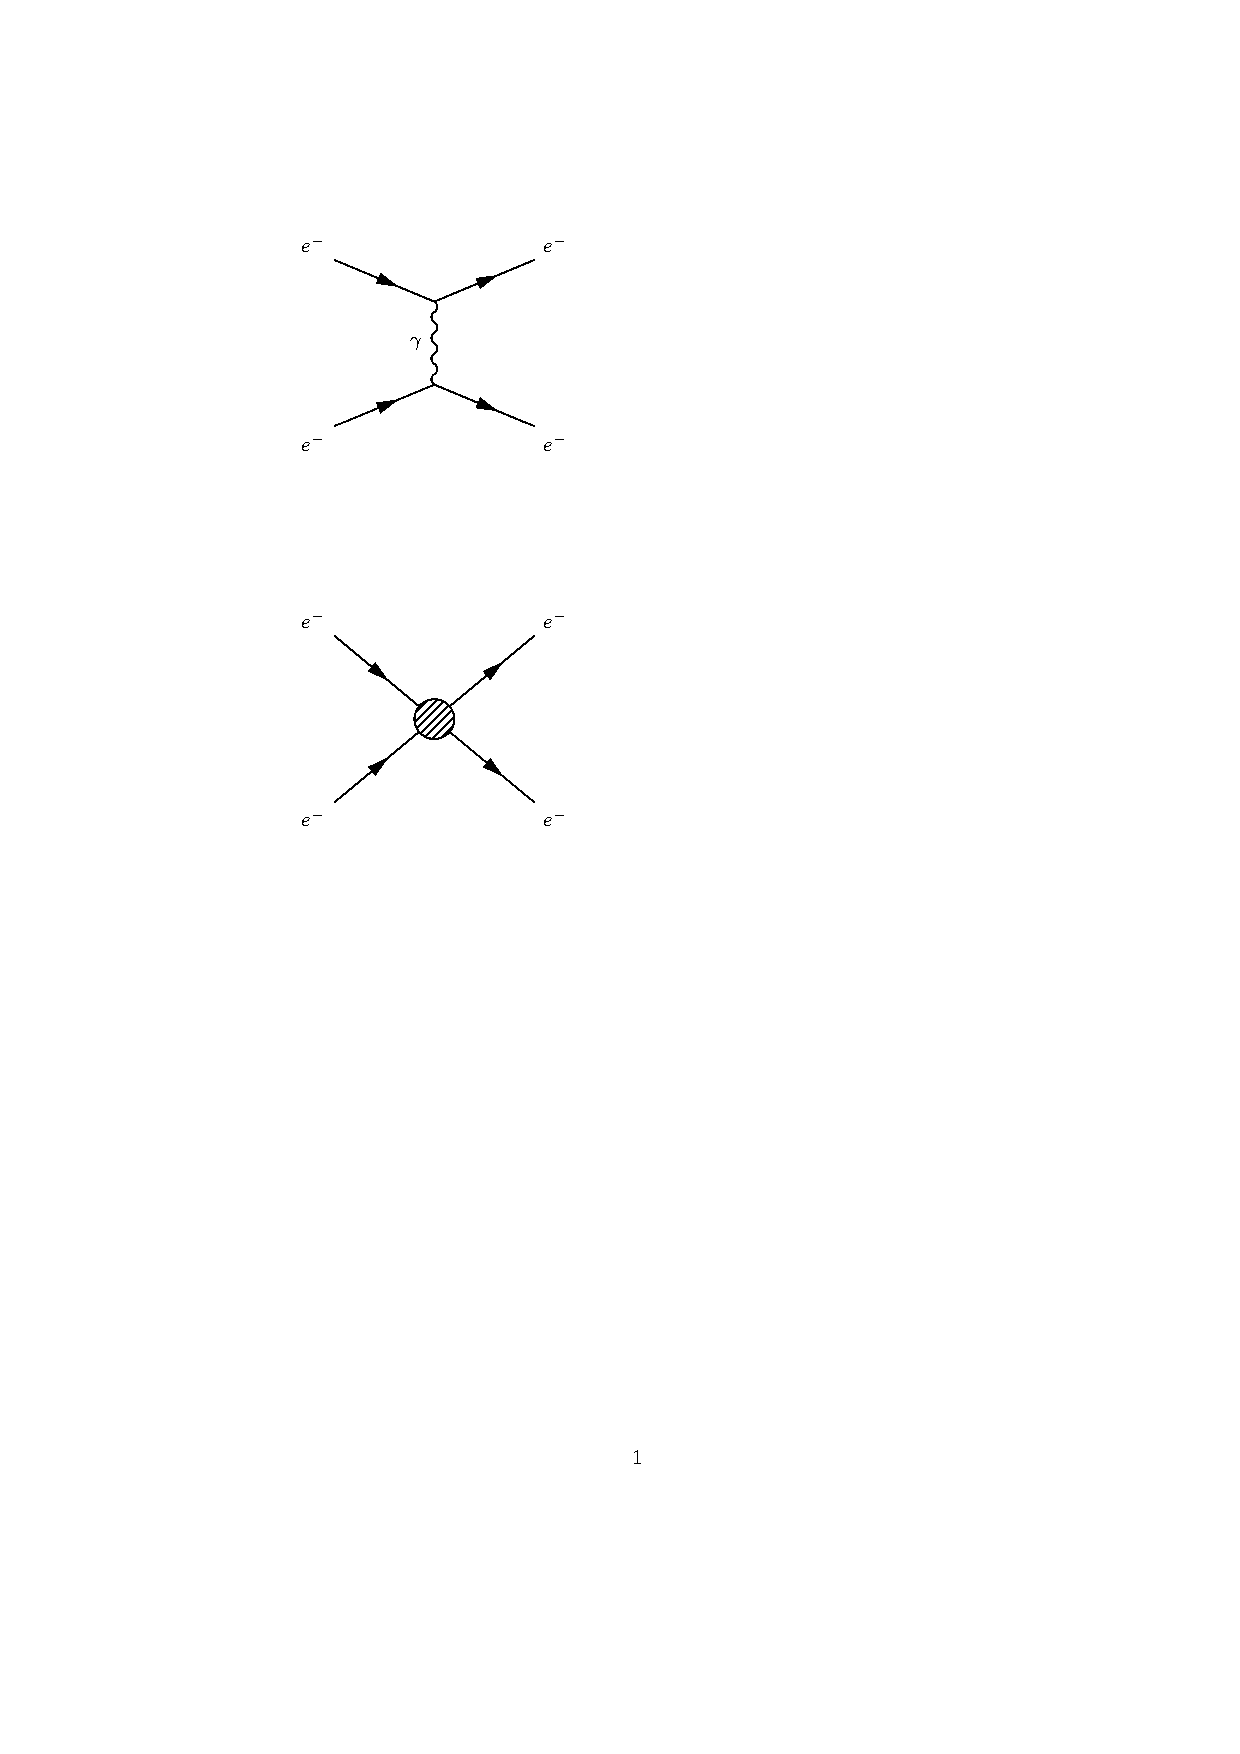
\includegraphics[trim=5cm 22cm 11cm 4cm,clip=true, width=0.4\textwidth]{myfeynman.pdf}
  \caption{{\small An example of a Feynman diagram explaining an electron-electron scattering using \abbrQED.}}
    \label{fig:exFeynman}
\end{SCfigure}

For a particle collision \citep{Herr:2006}, the cross-section can be seen as a measure of the effective surface area seen by the impinging particles and as such is expressed in units of area. The cross section is proportional to the probability that an interaction will occur. It also provides a measure of the strength of the interaction between the scattered particle and the scattering center. A step to simplify the calculation of the cross-sections is to use so called Feynman diagrams, an example of which is given in \figureref{fig:exFeynman}. Through the figure, which comes with certain rules, and knowing what the major process (in this case \abbrQED) one can calculate the cross-section \citep{Zee:2003,Herr:2006}. It is this which is needed to predict the detection of new particles. 

\subsection{Nuclear, particle and subatomic particle physics}\label{sec:tb:subsec:nps}
Many could argue that these branches of physics started after Ernest Rutherford famous gold foil experiment \citep{Burchan:1995}, where he discovered that atoms are composed of a nucleus, a lot of empty space and electrons. 

It was this that sparked the curiosity to see what the nucleus is made of and what forces govern the insides of atoms. After this, and the combination of the theoretical description given by \abbrQM, a lot more has been discovered and still more has been predicted. The newest of these is of course the Higgs particle, which was predicted through \abbrQFT and then discovered by the \abbrATLAS and the \abbrCMS experiments at \abbrCERN \citep{Higgs:2012, Chatrchyan:2012}. 

It is now known that all discovered particles are built up of fundamental particles, these build up the standard model \citep{Burchan:1995}.
\subsection{The standard model of particle physics}\label{sec:tb:subsec:SM}
To date there are two fundamental types of particles which are modelled as point like, quarks and leptons, seen in \figureref{fig:SM}. Aside from this and also seen in the figure are the gauge bosons which are mediators of the different forces.

All other known particles are built up by these fundamental particles. Combined particles are often divided into different groups depending on the fundamental particles that build them up. For instance, particles build up of three quarks are known as hadrons. Particles with an integer spin are known as bosons whereas half-integer particles are known as fermions.

The standard model of particle physics, referred to simply as the standard model (\abbrSM), categorizes all the fundamental particles that have been discovered experimentally. \abbrQFT explains the interactions between these particles and it has also predicted several particles by including symmetries \citep{Burchan:1995}.
\begin{figure}[h]
 \centering
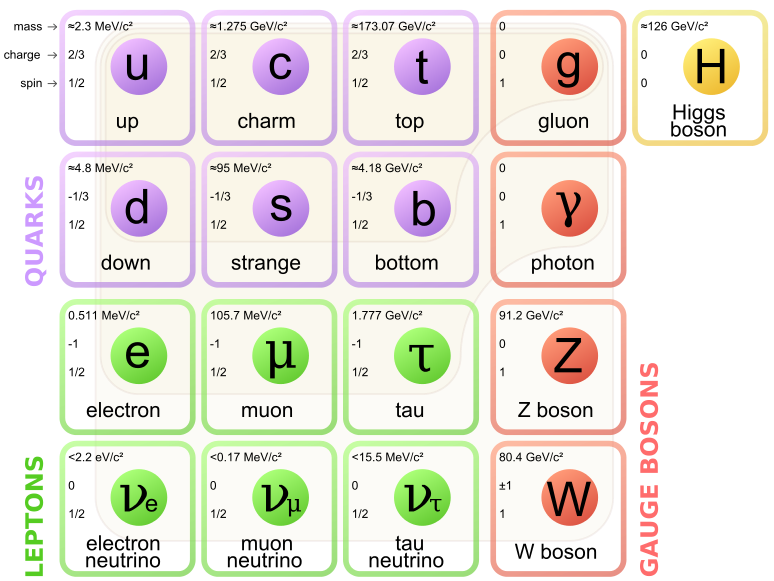
\includegraphics[width=\textwidth]{Standard_Model_of_Elementary_Particles.png}
  \caption{{\small The standard model of particle physics where the three first columns represent the so called generations, starting with the first \citep{wiki1}.}}
    \label{fig:SM}
\end{figure}

\abbrSM is today the pinnacle of particle physics and can be used to explain almost everything that occurs around us. There are however some problems \citep{Jungman:1996}:
\begin{itemize}
\item There is no link between gravity and the \abbrSM.
\item Asymmetry between matter and antimatter can not be fully explained.
\item No explanation that can contain dark matter.
\end{itemize} 
In this thesis focus lies with dark matter, some more introduction to possible dark matter and different candidates in extensions to \abbrSM are explained in \subsectionref{sec:tb:subsec:dark}.


\subsection{Dark matter}\label{sec:tb:subsec:dark}
Dark matter is the name given to, among other things, the solution to the discrepancies of galactic rotations \citep{darkmatter}.

The presence of dark matter can be measured indirectly from its gravitational effects. Focus on matter in a galaxy which is rotating around the center of the galaxy. Through Newtons law of gravity and the centrifugal force one can calculate the rotation speed as a function of the distance to the center of the galaxy. Since one of these forces is attractive and the other repulsive, if the matter is in a stable orbit around the galactic center they must be equal and give us an expression for the speed depending on the distance. Newtons law and the centrifugal force can be written as:
\begin{equation}\label{eq:forces}
F_{Gravitational}=G \frac{M m}{r^2} \equiv G_M \frac{m}{r^2} \qquad F_{Centrifugal} = m\frac{V^2}{r}
\end{equation}
where $G$ is the gravitational constant, $M$ the mass of the centre object, $m$ the mass of the matter, $r$ the distance between the two and $V$ is the rotation speed. It has been simplified using $G_M$ since all matter orbits the same galactic center. The assumption that the two objects have spherical symmetrical mass distributions and that the rotating object is in a circular orbit outside of the center object have been made. Setting the equations in \eqref{eq:forces} equal result in:
\begin{equation}\label{eq:rotation}
G_M \frac{m}{r^2} = m\frac{V^2}{r} \Leftrightarrow V^2 =\frac{G_M}{r} \Rightarrow V=\sqrt{\frac{G_M}{r}} \propto \frac{1}{\sqrt{r}}
\end{equation}
where the $V$ is assumed to be positive and $\propto$ denotes proportionality. Through these simple calculations it is shown that the rotation speed should decrease with and increased distance. The same reasoning can be applied to our solar system where this is the case, see \figureref{fig:rotation:a}. The relation for our solar system is in these units $V=\frac{107}{\sqrt{r}}$ where 107 can be used in \eqref{eq:rotation} to calculate the mass of the sun.

When applying the same reasoning to galaxies, the rotation speed does not decrease with an increased distance! In \figureref{fig:rotation:b} experimental data can be seen from the galaxy NGC3198 with a fitted curve which does not decrease with the distance but is instead constant.  This is the discrepancy which is solved by postulating the existence of dark matter \citep{1933AcHPh}.
 \begin{figure}[h] %!ht
    \subfloat[Rotation speed of planets in our solarsystem. Since the distance is quite small on an astronomical scale, there is no sign of dark matter. Based on data from Ref. \citep{Nasa}. \label{fig:rotation:a}]{%
     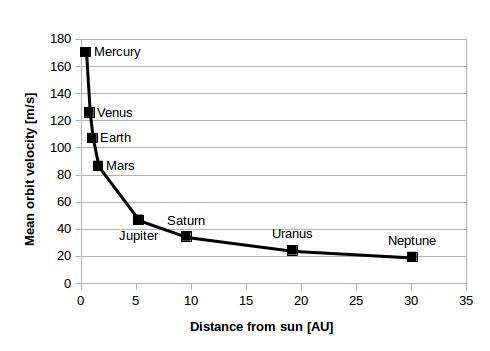
\includegraphics[width=0.5\textwidth]{solarsystemrotation2.jpg}
    }
    \hfill
    \subfloat[Rotation speed of mater in NGC3198 with a curve fitting and three different models, if only a dark model halo existed, if there was no dark matter and the correct, if both exist \citep{Albada:1985}.\label{fig:rotation:b}]{%
      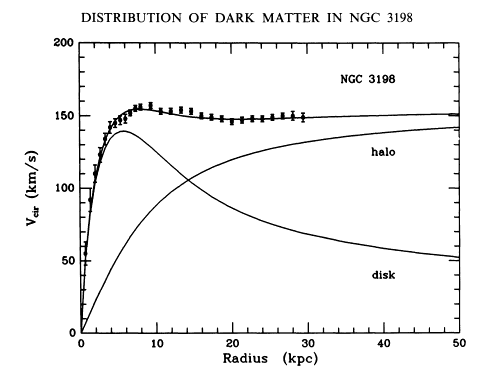
\includegraphics[width=0.5\textwidth]{rotationNGC3198.png}
    }
    \caption{Different rotation curves, both for planets in our solar system and matter in the NGC3198 galaxy.}
    \label{fig:rotation}
  \end{figure}
After this the big question arises, what could dark matter consist of? What is known so far lies in the name. It is called dark since there is no electromagnetic interaction and matter since it has gravitational interaction. This means that it can not be made up of anything in the Standard Model apart from neutrinos. Astrophysical measurements have also indicated that dark matter can not be fully explained as being neutrinos nor baryonic matter \citep{Gondolo:2003}. This means that dark matter can not be made out of any standard model particles. 

The main interest of this thesis and also the main contributor to the rotational discrepancies is known as cold dark matter. This is due to the matter having a low speed, thus low kinetic energy, and have a high particle mass (In the GeV scale) \citep{Goodman:2010,CERN-PH-EP-2012-210,Jungman:1996}.
There are several strategies to search for dark matter, \citep{Jungman:1996}.
\begin{itemize}
\item Ordinary matter interacting with ordinary matter can produce dark matter, known as production. This is the processes that occurs at particle accelerators is the method explored in this thesis.
\item Dark matter interacting with ordinary matter can produce dark matter, known as direct detection.
\item Dark matter interacting with dark matter can produce ordinary matter, known as indirect detection.
\end{itemize} 
In this thesis the focus lies with production at colliders, namely the \abbrLHC . There are several theoretical models for how to detect dark matter in proton-proton collisions such that occur at the \abbrLHC at \abbrCERN. This is covered more in \subsectionref{sec:tb:subsec:WIMPS}. 

\subsection{Signal models}\label{sec:tb:subsec:eft}
In quantum field theory the objective is usually to find the part of the Lagrangian which explains a type of interaction, known as the operator of the interaction and also to find the probability amplitude (cross-section) for a certain interaction. For complicated processes it is easier to employ a simplified phenomenological model. This is done by using an effective field theory and the concept is explained in \figureref{fig:feymanc}. The operator can be found through assuming the possible interactions and using the effective field theory \citep{Zee:2003}. 
%trim=left botm right top.
 % good for finding limits \fbox{\includegraphics}
 \begin{figure}[H] %!ht
    \subfloat[Electromagnetic interaction.\label{fig:feymanc:a}]{%
     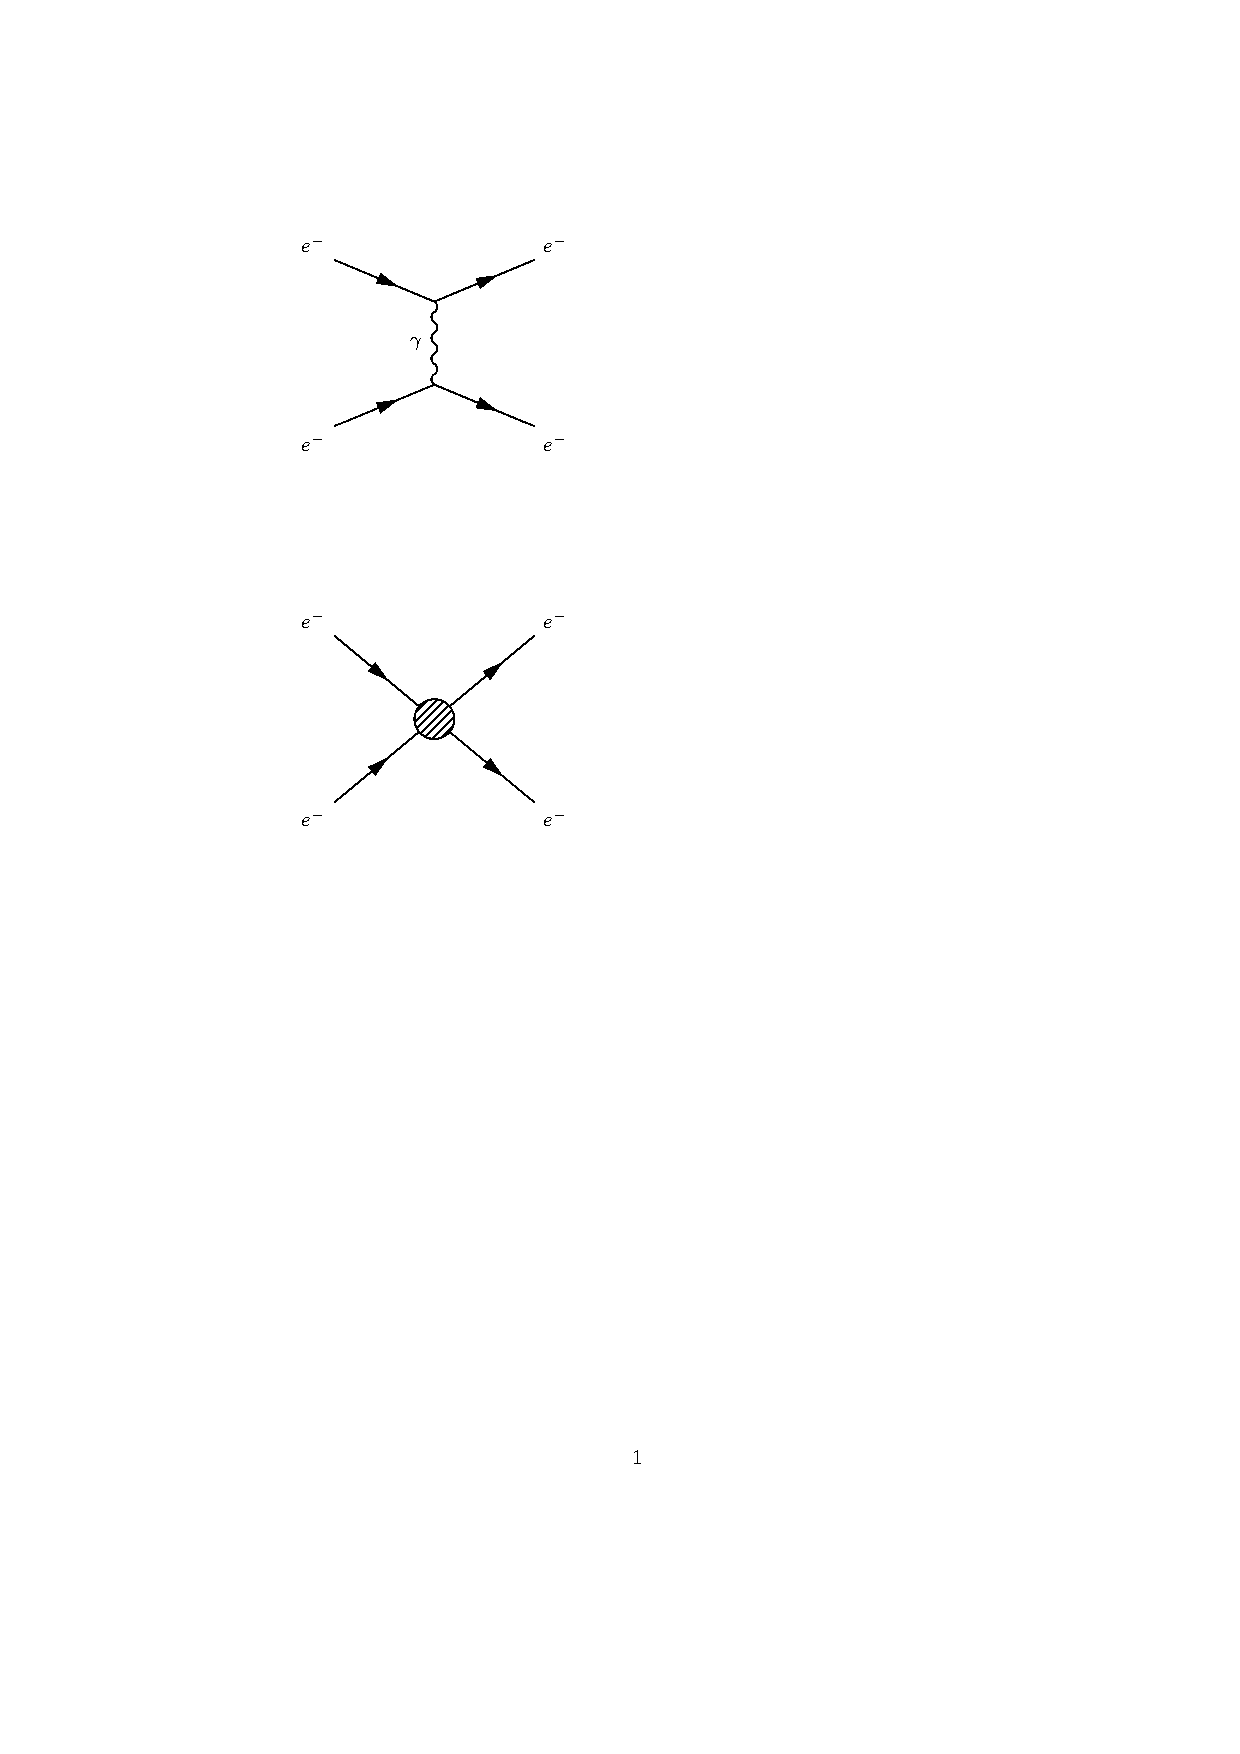
\includegraphics[trim=5cm 22cm 11cm 4cm,clip=true, width=0.5\textwidth]{myfeynman.pdf}
    }
    \hfill
    \subfloat[Effective diagram of \figureref{fig:feymanc:a}.\label{fig:feymanc:b}]{%
      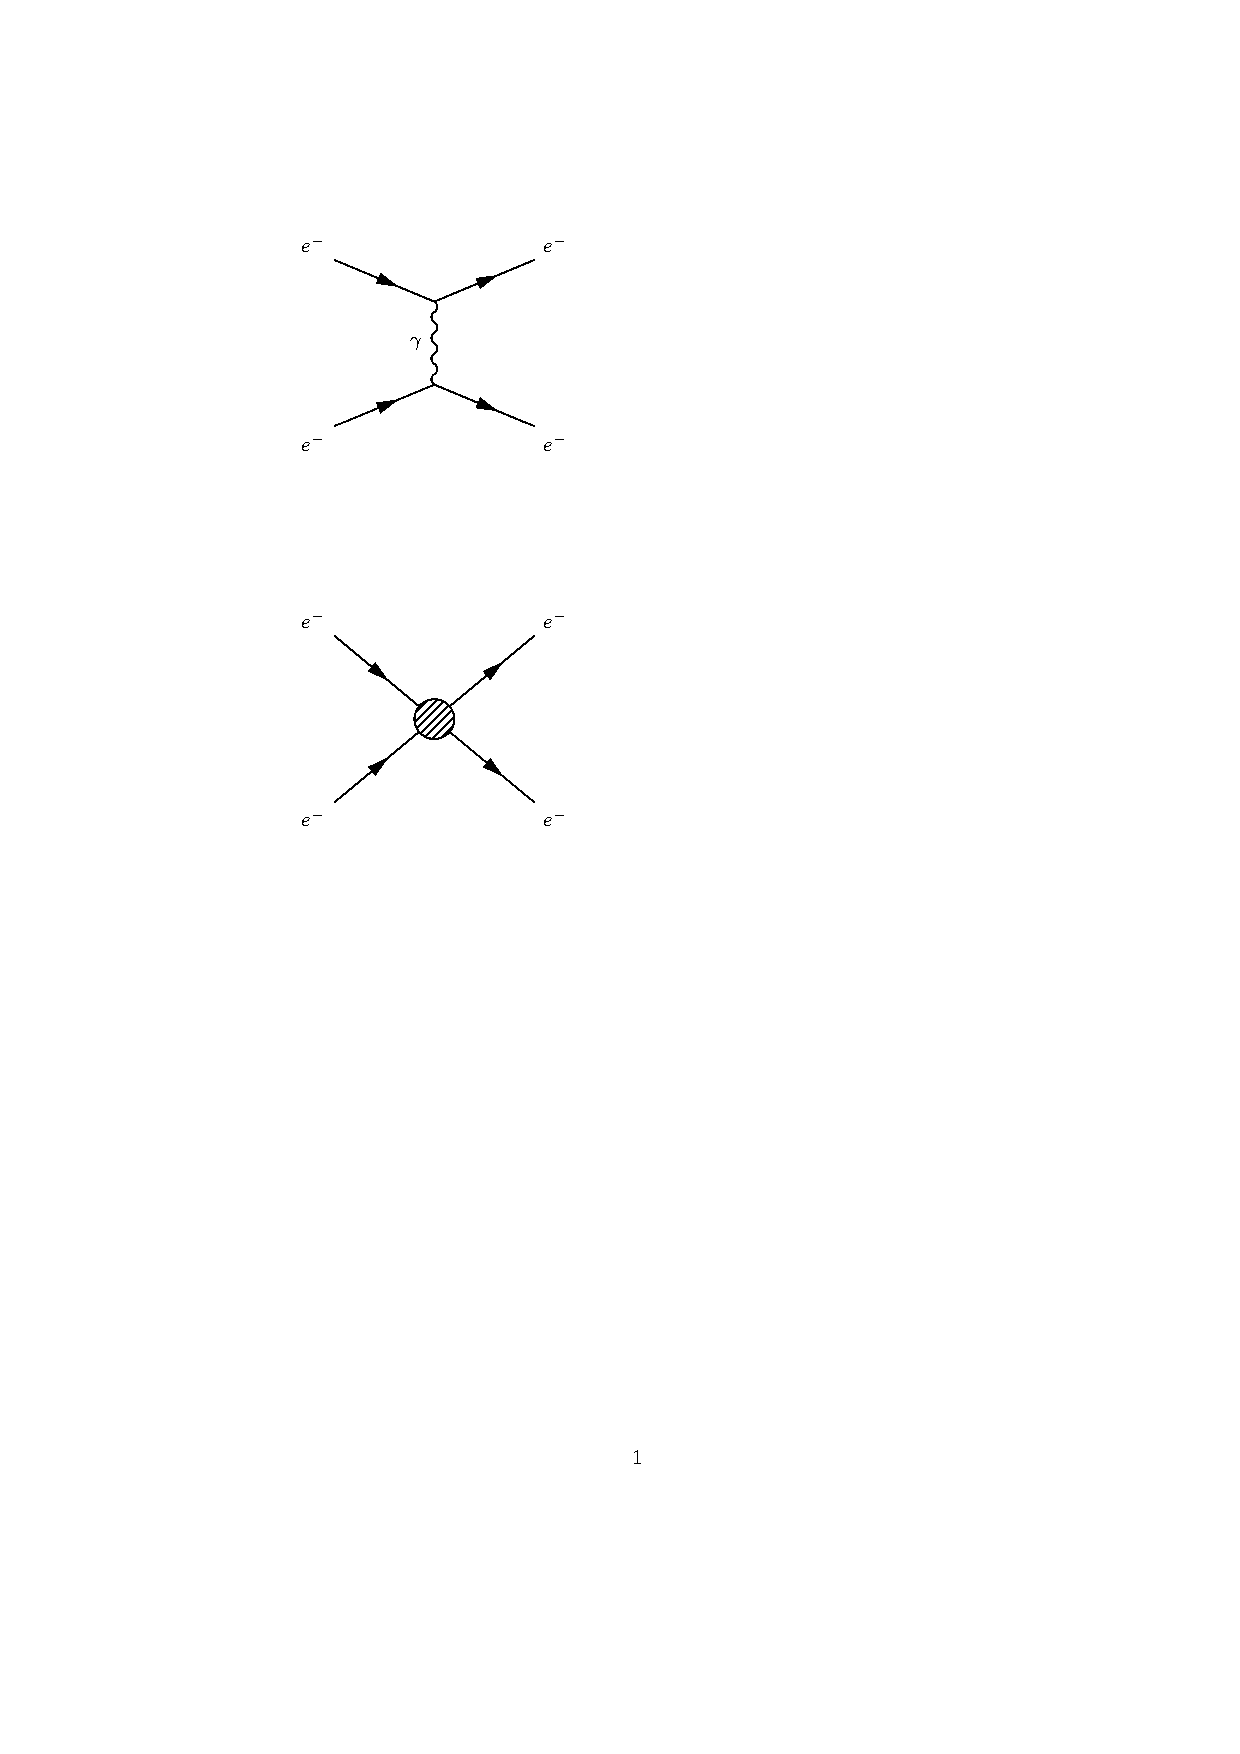
\includegraphics[trim=5cm 15.7cm 11cm 10.3cm,clip=true, width=0.5\textwidth]{myfeynman.pdf}
    }
    \caption{Feyman diagram of an electron-electron scattering, both as a diagram where a photon is exchanged and as its effective theory version, where the details are hidden in the blob.}
    \label{fig:feymanc}
  \end{figure}
In this thesis the same effective field theory as in Refs. \citep{82.116010,Goodman:2010} is considered, denoted D5 and explained in \figureref{fig:opfeyn:a}. The \abbrWIMP (denoted $\chi$) is assumed to be the only particle in addition to the standard model fields and is assumed to interact through the electroweak force. In order to explain dark matter the \abbrWIMP $\chi$ must be stable, for this reason only Feynman diagrams with an even number of $\chi$ are considered. It is assumed that the mediator is heavier that the \abbrWIMPS, meaning that the mediator interactions are in higher order terms of the effective field theory and thus not included in the operators. In this work, WIMPS are assumed to be Dirac fermions (half integer spin and is not its own antiparticle). 

Another model which is considered is a vector mediator model which is described by \figureref{fig:opfeyn:b}. This model is based on the assumption that the interaction of \abbrWIMPS is mediated by a particle denoted V which is a spin 1 particle. This particle is modelled as a heavy z-boson which governs the electroweak interactions. The free parameters of this mediator particle are its weight and its width which is related to the lifetime of the particle and which decay modes exist. 

 \begin{figure}[H] %!ht
    \subfloat[Effective Feynman diagram explaining the D5-operator. \label{fig:opfeyn:a}]{%
     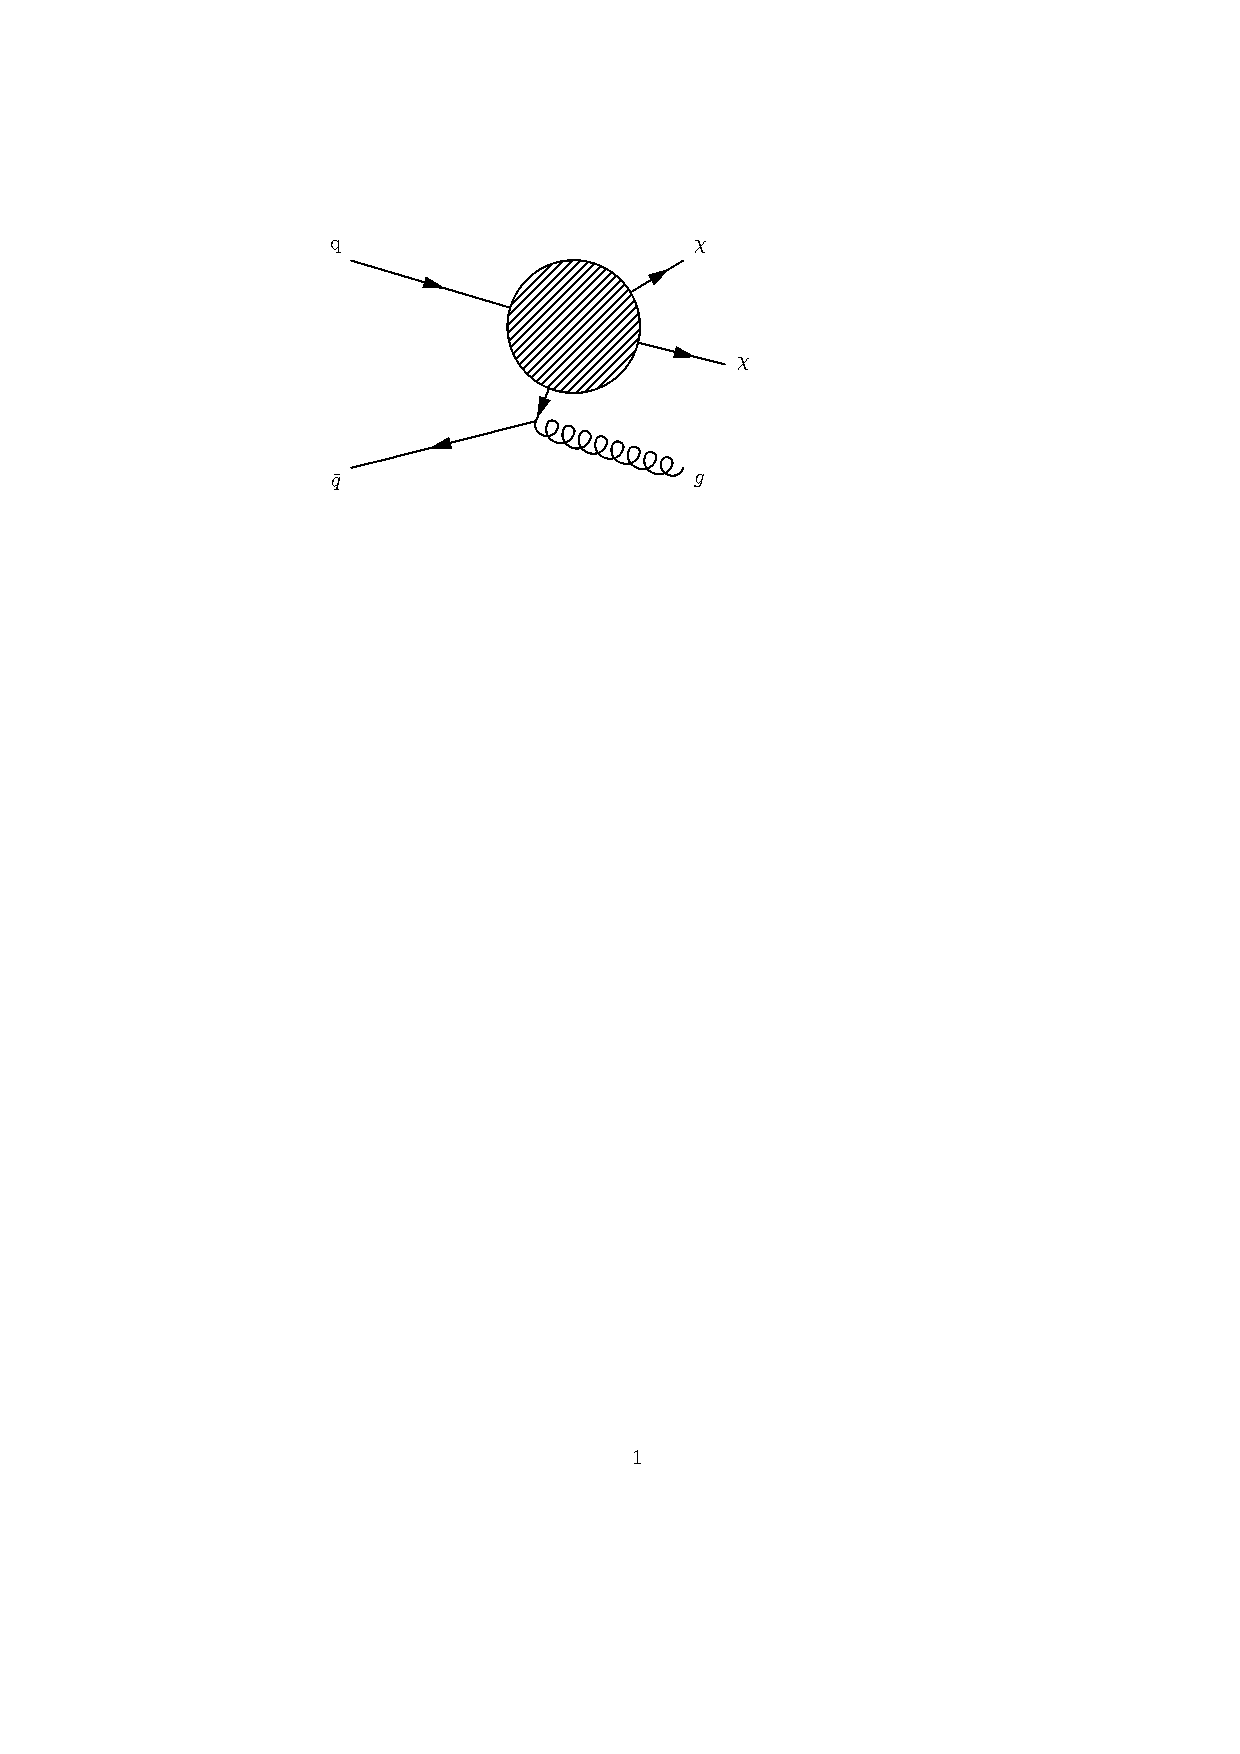
\includegraphics[trim=5cm 21cm 8cm 3.9cm, clip=true, width=0.5\textwidth]{effectiveD.pdf}
    }
    \hfill
    \subfloat[Feynman diagram describing the vector mediator model. \label{fig:opfeyn:b}]{%
      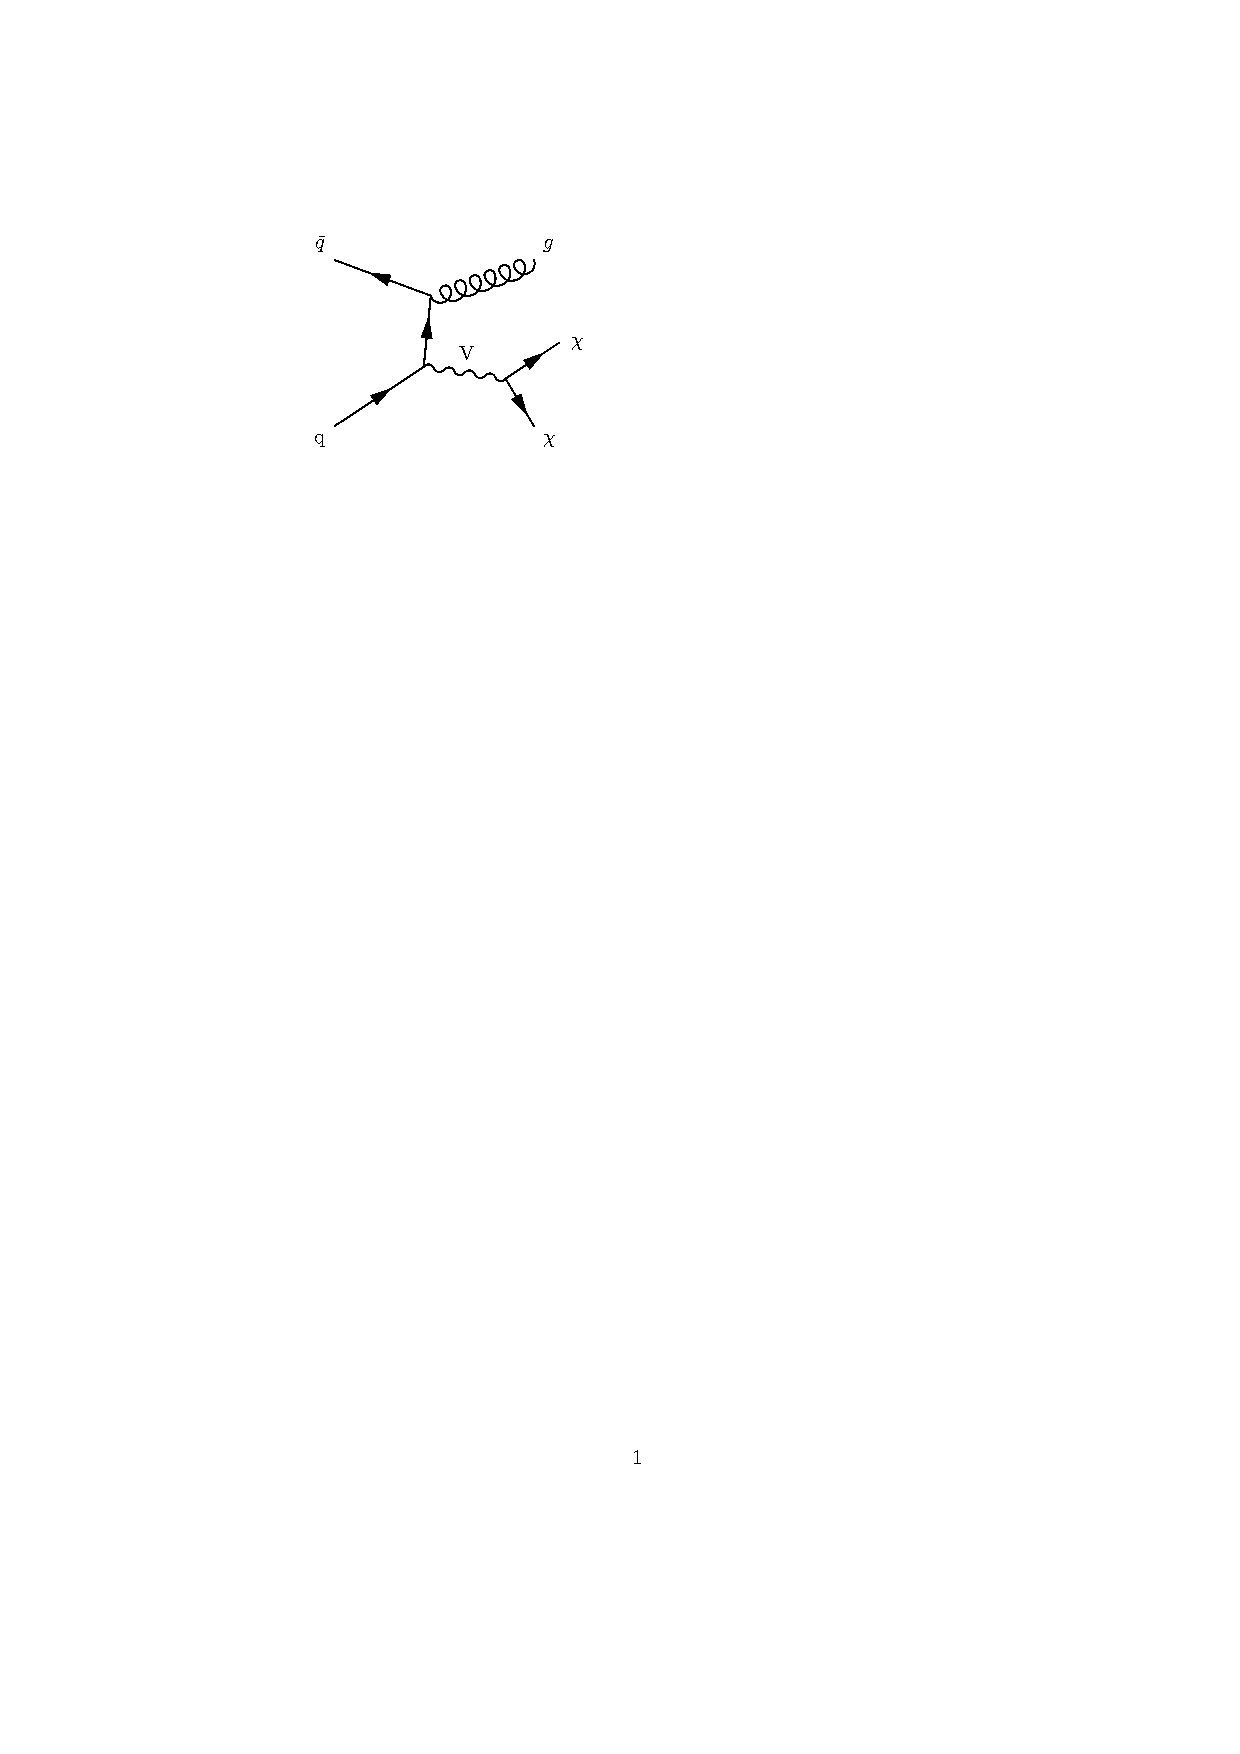
\includegraphics[trim=5cm 22cm 10cm 3.9cm, clip=true, width=0.5\textwidth]{vectorboson.pdf}
    }
    \caption{Feynman diagrams describing the signal models used in this thesis.}
    \label{fig:opfeyn}
  \end{figure}


\subsection{Jets}\label{sec:tb:subsec:jets}
In particle collisions free gluons and quarks with high energy can be produced. According to \abbrQFT these can not exist and must decay through a process known as hadronization meaning that they will decay into a cone of energetic hadrons, which is known as a Jet. It is not possible to measure these free gluons or quarks, however this cone of hadrons will travel in the same direction and will be measured by the calorimeters, see \subsectionref{ATLAS}. These measurements can then be summed to calculate the energy and momentum which the initial gluon or quark had which in turn results in more information about the collision.

\subsection{Search for \abbrWIMPS}\label{sec:tb:subsec:WIMPS}
The main problem with searching for \abbrWIMPS is that one is looking for a small signal among a lot of uninteresting proton-proton collisions. One way to search for \abbrWIMPS and overcome this difficulty is a so called mono-jet analysis which is described in \subsectionref{sec:eo:subsec:mjet}. 

This method is a way to detect \abbrWIMP production among other proton-proton collision events and relies on the observation of high energetic jet, which arises from the gluon in both figures in \figureref{fig:opfeyn}, on one side and seemingly non conservation of energy or momentum, which will be denoted missing energy. This means that something has happened which the detectors can not detect. If the models from \subsectionref{sec:tb:subsec:eft} can explain the missing energy, then evidence for \abbrWIMP production would have been found.

Since the search for \abbrWIMPS at the \abbrLHC is based on looking at the missing energy, not actual detection, the experiment can not establish if a \abbrWIMP is stable on a cosmological time scale and thus if it is a dark matter candidate \citep{CERN-PH-EP-2012-210}. This means that if a candidate is found, it may still not be the dark matter that is needed to explain the cosmological observations.

ATLAS has looked at proton-proton collisions, with 8 TeV center of mass energy, which contain high energetic jets, without finding any excess of mono-jet events. This is why it is very interesting that the \abbrLHC is undergoing a upgrade that will allow higher energy levels, see \subsectionref{sec:eo:subsec:hlu}. With this collisions can be given higher energy and thus the produced particles can be comprised of higher mass. 
\newpage
\section{Experimental overview}\label{sec:experiment}
\subsection{\abbrLHC}
The large hadron collider (\abbrLHC) is a particle accelerator located at \abbrCERN near Geneva in Switzerland, see \figureref{fig:lhc}. The accelerator was built to explore physics beyond the standard model and to make more accurate measurements of standard model physics. Before it was shut down for an upgrade in 2012 it was able to accelerate two proton beams to such a velocity that each proton in them had an energy of 4 TeV which gives a center of mass energy of $\sqrt{s}=8$ TeV. The proton beam is comprised of bunches of protons with enough spacing that bunch collisions can happen independent of each other. The rate at which the accelerator produces a certain process can be calculated through the instantaneous luminosity. For the \abbrLHC the instantaneous luminosity was $10^{34}$ cm$^{-2}$s$^{-1}$ \citep{lumires} or $10$nb$^{-1}$s$^{-1}$ where 1 barn(b)$=10^{-24}$ cm$^2$.
\begin{figure}[H]
\begin{center}
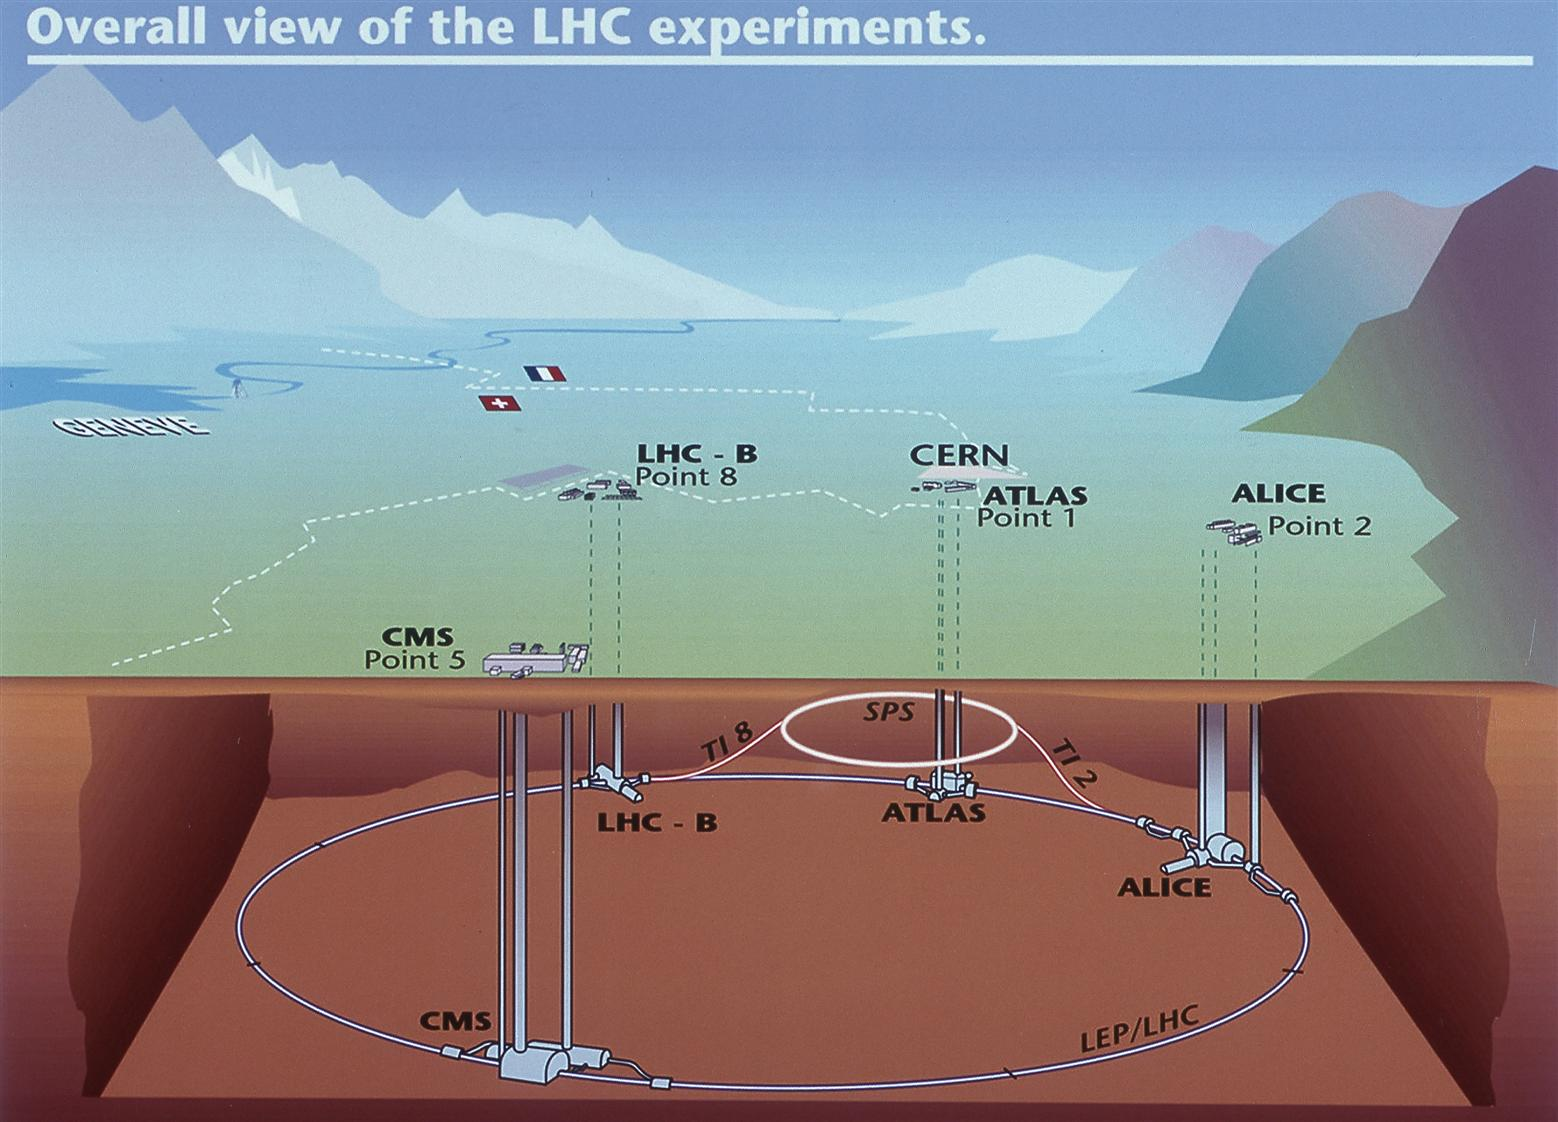
\includegraphics[width=\linewidth]{lhc.jpeg}
\caption{The \abbrLHC and the different detector sites \citep{lhcimage}.}
\label{fig:lhc}
\end{center}
\end{figure}
The instantaneous luminosity, often just denoted luminosity, can be defined in different ways depending on how the collision takes place. For two collinear intersecting particle beams it is defined as:
\begin{equation}\label{eq:instl}
\mathscr{L} = \frac{fkN_1 N_2}{4\pi \sigma_x \sigma_y}
\end{equation}
where $N_i$ is the number of protons in each of the bunches, f is the frequency at which the bunches collide , k the number of colliding bunches in each beam, and $\sigma_x$ ($\sigma_y$) is the horizontal (vertical) beam size at the interaction point. Since the instantaneous luminosity increases quadratically with more protons in each bunch, increasing the number of protons would be a good strategy to increase the instantaneous luminosity. However aside from the difficulties to create and maintain a beam with more particles, a large $N_i$ increases the probability for multiple collisions per bunch crossing, referred to as pile-up. Pile up will be a key aspect which is described more in \subsectionref{sec:eo:subsec:pile}. 

The expected number of events for a given physical process can be calculated by using the instantaneous luminosity \eqref{eq:instl} through the following:
\begin{equation}\label{eq:Numevents}
N=\sigma \int \mathscr{L} dt \equiv \sigma \Lagr
\end{equation}
where $\Lagr$ is the integrated luminosity and $\sigma$ is the cross section which is often measured in barn.
The integrated luminosity is a measurement of total number of proton-proton interactions that have occurred over time and is also a common measure of how much data was recorded. Before the \abbrLHC was shut down $\Lagr$ was 20.8 fb$^{-1}$.

\subsection{\abbrATLAS}\label{ATLAS}
As seen in \figureref{fig:lhc}, there are several detectors at the \abbrLHC. One of these is \abbrATLAS which is a general purpose detector that uses a toroid magnet. Its goal is to observe several different production and decay channels. The detector is composed of three concentric sub-detectors, the Inner detector, the Calorimeters and the Muon spectrometer \citep{1129811}.

The Inner detectors main task is to measure the tracks of the particles and measure the position of the initial proton-proton collision. Aside from this it measures the track momenta and the charge of charged particles. It can however only detect charged particles.

The Calorimeters, electromagnetic and hadronic, are used to measure the energy contained in the different particles. The electromagnetic calorimeter is used to measure energy and direction of photons and electrons whereas the hadronic calorimeter is designed to measure the energy and direction of hadrons.

The Muon spectrometer is used to measure signs of muons, which will simply pass through the other detectors without leaving a trace. It also measures the energy and momentum of the muons.

The neutrinos escape the \abbrATLAS experiment without being detected, and in this thesis it is assumed that \abbrWIMPS pass through all the detectors without leaving any trace.

Therefore WIMPS and neutrinos have the same detector signature. As seen in \sectionref{chap:sig:sec:res} the main background to the WIMP signal is the production of a Z boson that in turn decay to two neutrinos mimicking the WIMP signature.
\subsection{Coordinate system}\label{sec:eo:subsec:coord}
The coordinate system of ATLAS, seen in \figureref{fig:coordinatesystem} is a right-handed coordinate system with the x-axis pointing towards the centre of the LHC ring, and the z-axis along the tunnel/beam (counter clockwise) seen from above. The y-axis points upward. The origin is defined as the geometric center of the detector. A cylindrical coordinate system is also used for the transverse plane, (R,$\varphi$,Z).
For simplicity the pseudorapidity of particles from the primary vertex is defined as:
\begin{equation}
\eta = - \ln( \tan\frac{\theta}{2})
\end{equation}
where $\theta$ is the polar angle (xz-plane) of the particle direction measured from the positive z-axis. The difference in $\eta$ of two particles is through this definition invariant under Lorentz boosts in the z-direction.

It is quite common to calculate the distance between particles and jets in the $(\eta,\varphi$) space, $d=\sqrt{(\Delta \eta)^2 + (\Delta \varphi)^2}$. 

\begin{figure}[ht]
\begin{center}
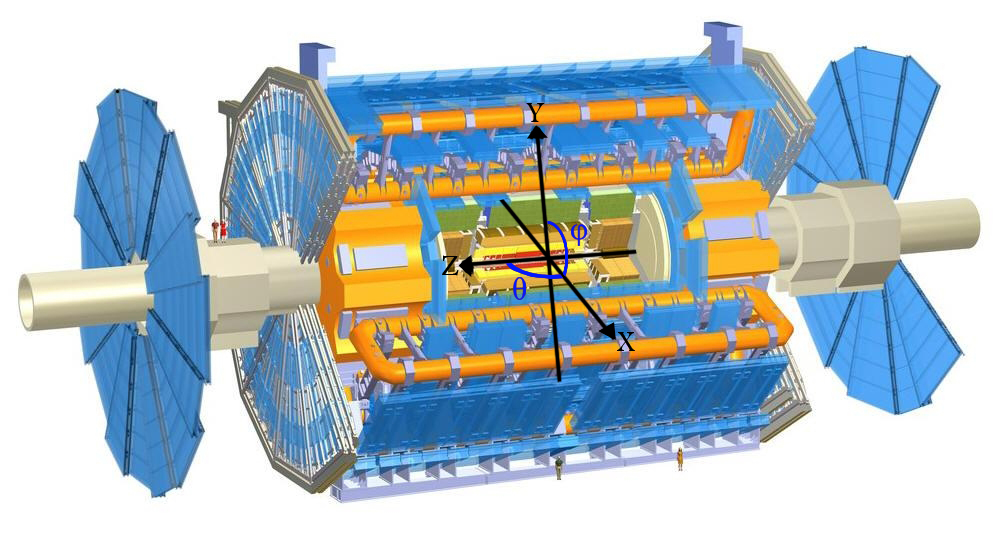
\includegraphics[width=\linewidth]{particle_collider.jpg}
\caption{The \abbrATLAS detector and the definition of the orthogonal Cartesian coordinate system. Image altered from Ref. \citep{coordimage}.}
\label{fig:coordinatesystem}
\end{center}
\end{figure}

\subsection{Pile-up}\label{sec:eo:subsec:pile}

Pile-up is the phenomena that several proton-proton collisions occur simultaneously. The number of pile-up is defined as the average number of proton-proton collisions that occur per bunch crossing per second. It is denoted as $\obs{\mu}$. $\mu$ can be calculated by adjusting a Poisson distribution to fit the curve created by the number of interactions per bunch crossing at a given luminosity. When this is done $\mu$ will be the mean value of the Poisson distribution. The value of $\mu$ will be higher for after the proposed upgrade compared to now, see \sectionref{sec:eo:subsec:hlu} which may decrease the detector performance.

\subsection{Mono-jet analysis}\label{sec:eo:subsec:mjet}

\begin{figure}[ht]
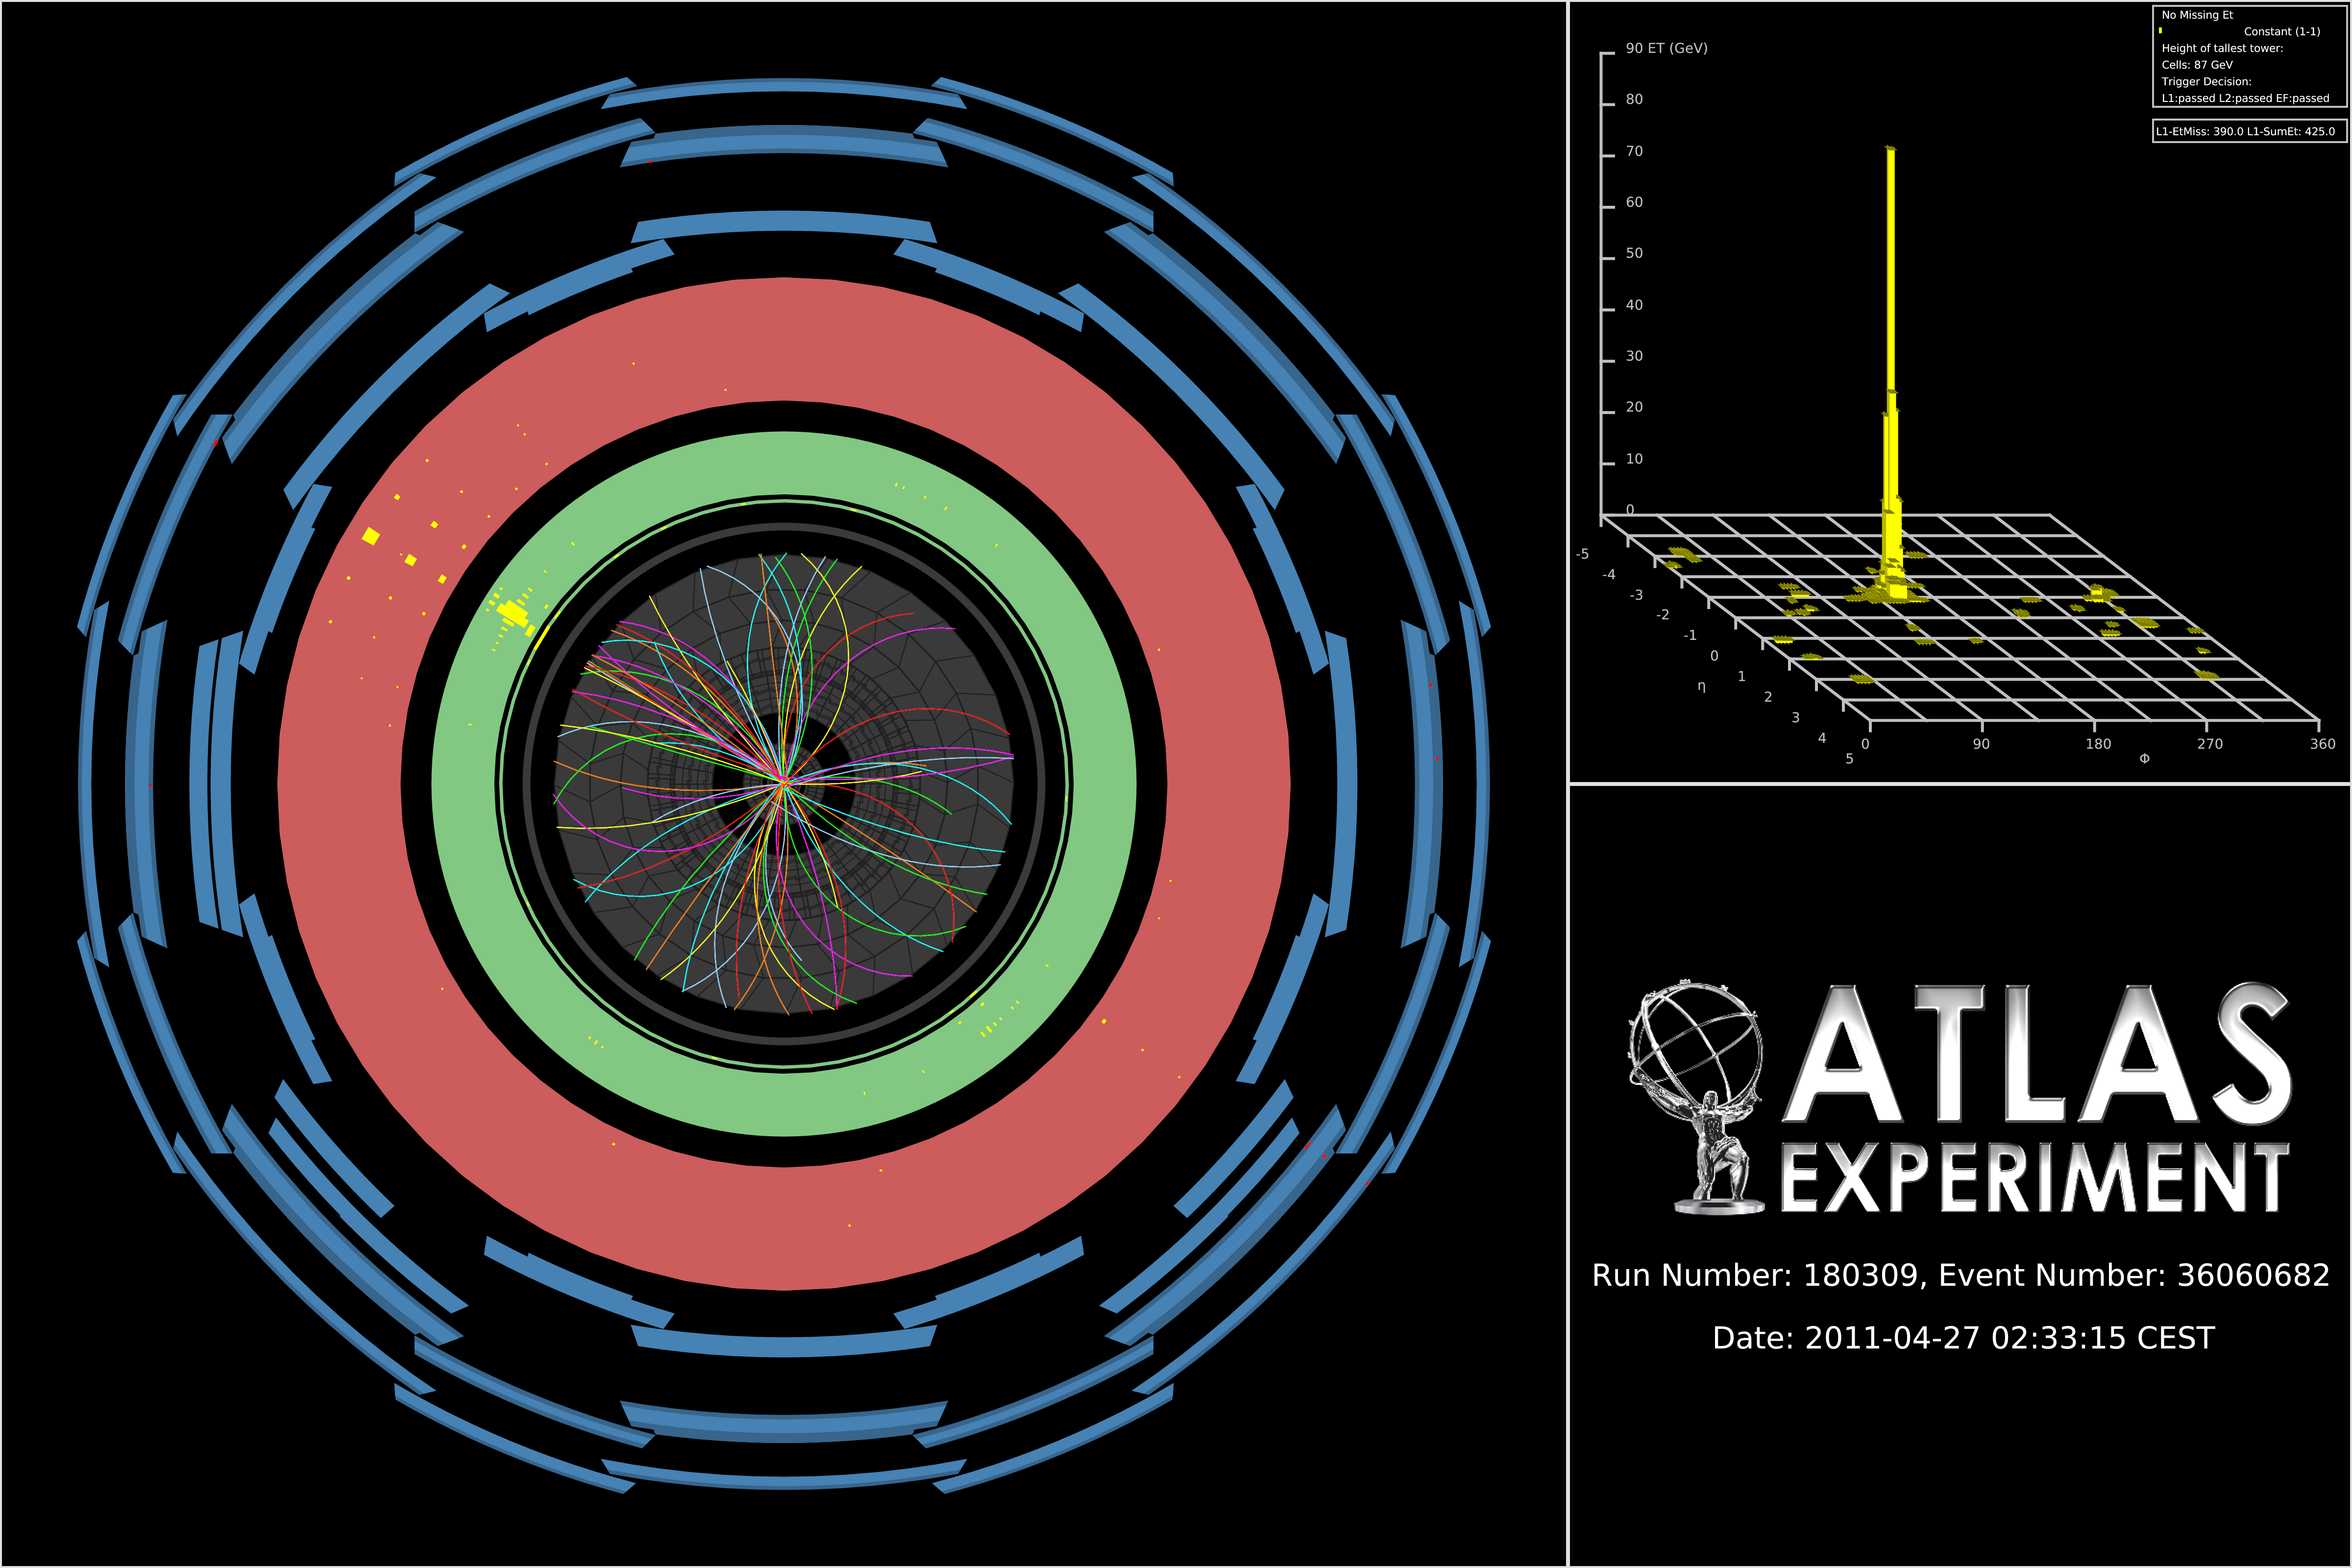
\includegraphics[width=\linewidth]{monojetbig.png}
\caption{Image in the transverse plane of a mono-jet event recorded by the \abbrATLAS experiment \citep{monojet}. The figure in the top right is a diagram in the $(\eta,\varphi)$-plane showing where in the calorimeter (red in the main figure) the energy is deposited and how much.}
\label{fig:monojet}
\end{figure}

When measuring the transverse energy one can in some interactions find inconsistencies such as jets, discussed in \subsectionref{sec:tb:subsec:jets}, that are in excess in one direction. Conservation of momentum in the transverse plane of the experiment indicates that the sum of all momenta should be zero as before the collision. In \figureref{fig:monojet} one can see a high energetic jet which gives an excess of transverse energy in one direction after the collision. Since there is no balancing jet there must be transverse energy that is not detected, denoted $E_T^{Miss}$. This gives an indication that the energy to balance this can not be detected. This could for instance be neutrinos or the characteristic signature of \abbrWIMPS .

$E_T^{Miss}$ is the modulus of the $E_T^{Miss}$ vector which is defined as:
\begin{equation}\label{eq:etmiss}
\vec{E_T}^{Miss} = - \sum \vec{p_T}^{Jet} - \sum \vec{p_T}^{Electron} - \sum \vec{p_T}^{Muon} - \sum \vec{p_T}^{Tau} - \sum \vec{p_T}^{Photon}
\end{equation}  
where $p_T$ denotes the transverse momenta.
There are two main classes of events, signal and background. 
The signal corresponds to events that would arise from one of the processes in \subsectionref{sec:tb:subsec:eft}. However to know that the missing energy is a sign of the signal then one must understand all the other components that could contribute to the missing energy. Also there must be an excess of missing energy from what is expected from the background this since the background comprises of standard model processes that can mimic the mono-jet signature.
\subsection{Phase II high luminosity upgrade}\label{sec:eo:subsec:hlu}
At the moment, the whole \abbrLHC is undergoing a step by step upgrade program which be finalized around 2022-2023, denoted the high luminosity upgrade, or HL-upgrade. The upgrade consists of different stages, meaning that the upgrade will halt for periods so that experiments can take place. 
\begin{figure}[ht]
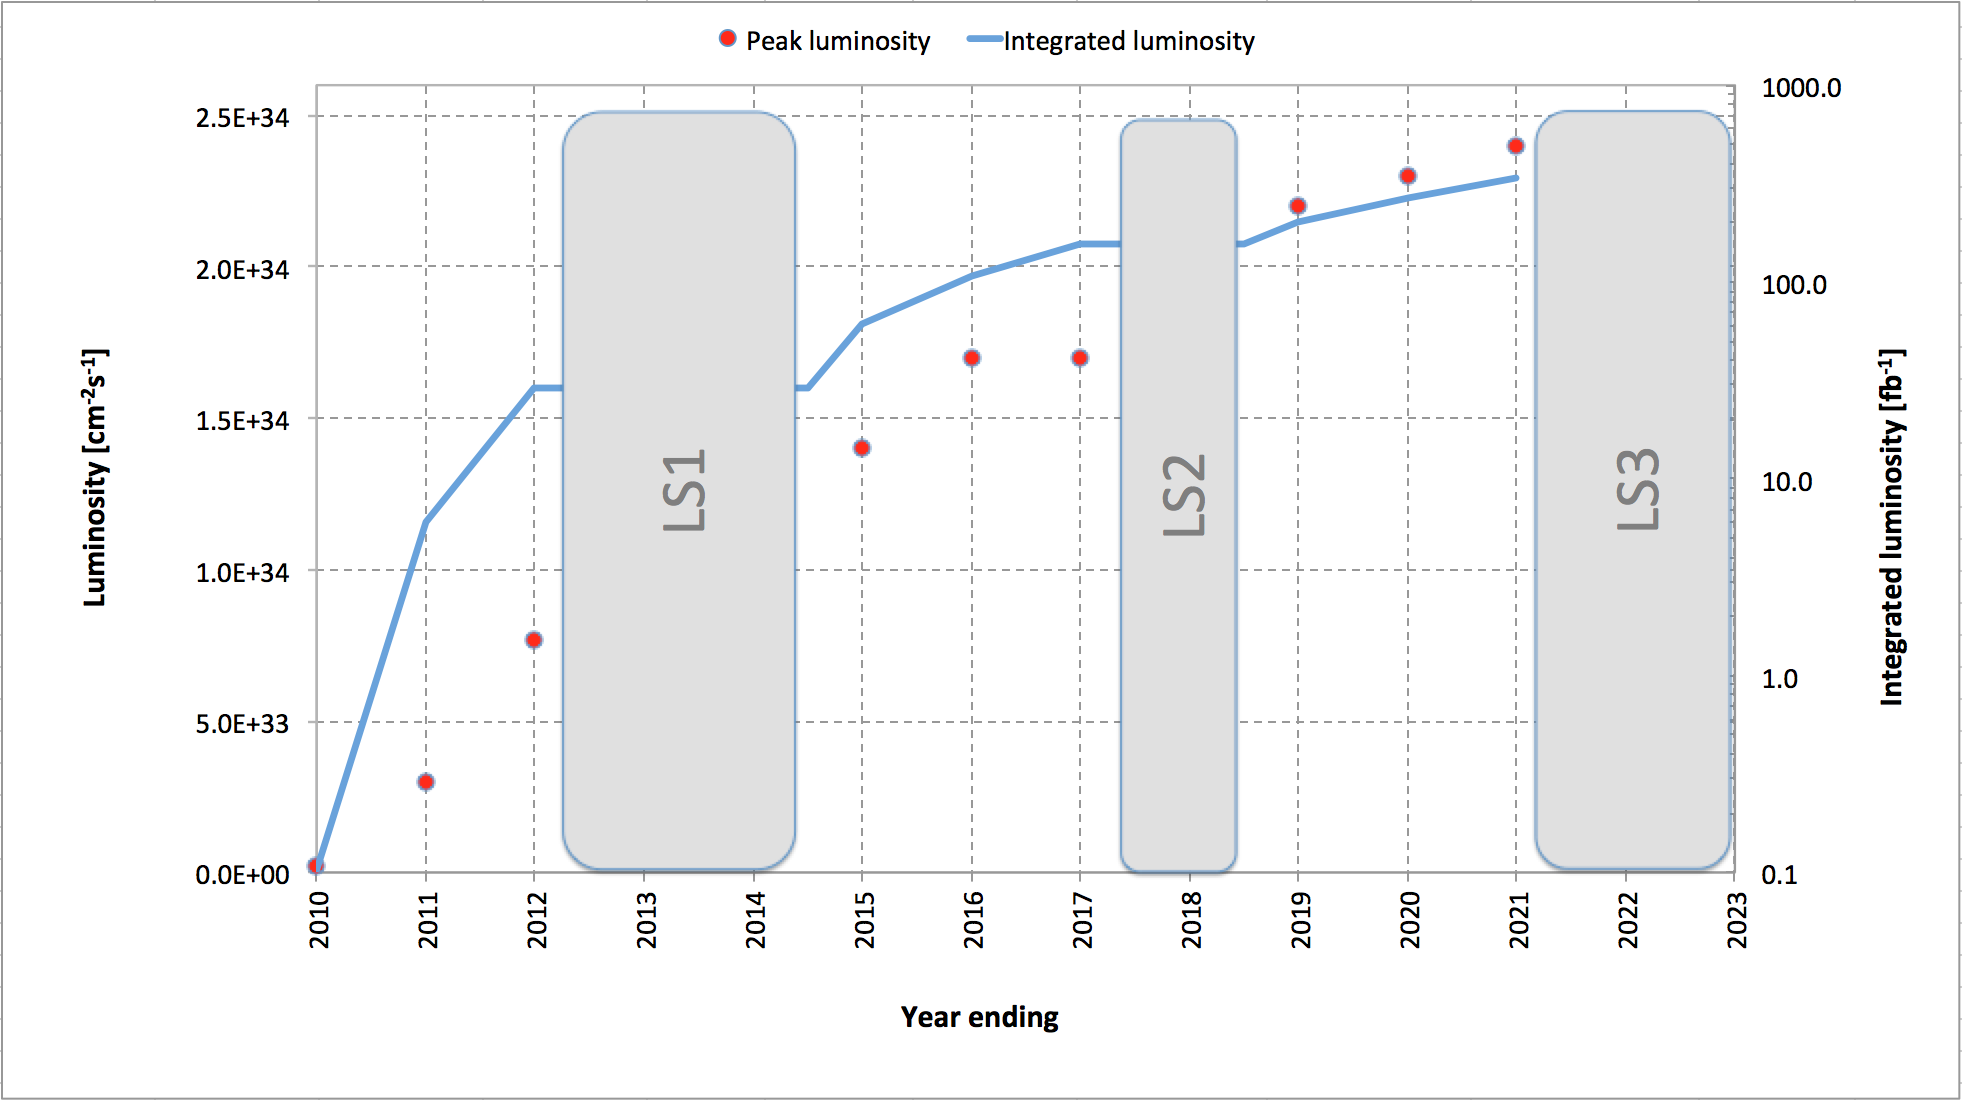
\includegraphics[width=\linewidth]{lumi-projection.png}
\caption{A graph showing the upgrading timetable with the instantaneous luminosity, denoted luminosity, and integrated luminosity expected in the different stages.}
\label{fig:upgt}
\end{figure}
In \figureref{fig:upgt} one can see the three proposed upgrades. The period after LS1 is denoted phase 0, after LS2 phase I and after LS3 phase II. 
\begin{itemize}
\item[LS1] is the upgrade which will take the \abbrLHC to its designed performance. 

\item[LS2] will push the LHC to the ultimate designed instantaneous luminosity without too dramatic changes to the accelerator. 
\item[LS3] which is the focus of this thesis, will increase the instantaneous luminosity even more. Though for this to happen a modification of the whole \abbrLHC must be done, instead of just an upgrade and maintenance as before.
\end{itemize}
The following is expected for the experiments done after phase II:
\renewcommand{\arraystretch}{1.5} %Change height of tabel
\begin{table}[H]
\begin{center}
    \begin{tabular}{ | l | l | l |}
    \hline
    Entity & Expected & Last run (2012) \\ \hline
    Instantaneous luminosity & $\mathscr{L}$ \textasciitilde 50 nb$^{-1}$s$^{-1}$ & $\mathscr{L}$ \textasciitilde 10 nb$^{-1}$s$^{-1}$ \\ \hline  
    Integrated luminosity & $\Lagr=1000-3000$ fb$^{-1}$ & $\Lagr=20$ fb$^{-1}$ \\ \hline
  	Pile-up & $\obs{\mu}=140$ & $\obs{\mu}=20$ \\ \hline
  	Center of mass energy & $\sqrt{s}=14$ TeV &  $\sqrt{s}=8$ TeV \\ \hline
  	\end{tabular}
  	
  	\caption{Expected running values for the Phase II HL-upgraded \abbrLHC with older values for comparison \citep{HL:2013}.}
  	\label{tab:expectvalues}
  	\end{center}
    \end{table}
    \renewcommand{\arraystretch}{1.0}  %Back to default
Where it should be noted that the integrated luminosity indicates the total amount of data which will be collected after the upgrade is completed before the next upgrade takes place. 

\subsection{Monte Carlo simulation}
As mentioned before, in this thesis only emulated data was used. This data is created by using a Monte Carlo (\abbrMC) simulation of the background processes and the expected signal. To do this a program called MadGraph is used.

MadGraph \citep{madgraph} starts with Feynman diagrams and then generates simulated events based on lots of different parameters. This generator was used to generate signal samples used in this thesis. 

Sherpa \citep{sherpa} is very similar to MadGraph and was used to generate the background samples used in this thesis.

PYTHIA \citep{Sjostrand:2008} is a package which adds the correct description of jets to MadGraph by including hadronization. The correct description of pile-up comes from other \abbrATLAS software.

The tool to access all this data and analyse it a tool called ROOT, which is used for programming high energy physics related tools \citep{root}.